\documentclass{tufte-handout}

\title{Section 5.3: Trigonometric Graphs}

\author[AW]{Ammon Washburn}

\usepackage{graphicx} % allow embedded images
  \setkeys{Gin}{width=\linewidth,totalheight=\textheight,keepaspectratio}
  \graphicspath{{graphics/}} % set of paths to search for images
\usepackage{amsmath}  % extended mathematics
\usepackage{booktabs} % book-quality tables
\usepackage{units}    % non-stacked fractions and better unit spacing
\usepackage{multicol} % multiple column layout facilities
\usepackage{lipsum}   % filler text
\usepackage{enumerate}
\usepackage{wrapfig}
\usepackage{fancyvrb} % extended verbatim environments
  \fvset{fontsize=\normalsize}% default font size for fancy-verbatim environments
\usepackage{tikz}
\usepackage{subcaption}
\captionsetup{compatibility=false}
\usepackage{mathtools}
\usepackage{graphicx}
\usepackage{amssymb}
\usepackage{enumerate}
\usepackage{color}
\usepackage{fancyvrb}
\usepackage{breqn}
\usepackage{fancyhdr}
\usepackage{multicol}
%\usepackage[latin1]{inputenc}
\usepackage{tikz}
\usepackage{pgfplots}
\pgfplotsset{compat=1.8}

\definecolor{dkgreen}{rgb}{0,0.6,0}
\definecolor{gray}{rgb}{0.5,0.5,0.5}
\definecolor{mauve}{rgb}{0.58,0,0.82}

\newcommand{\R}[1]{\mathbb{R}^{#1}}

\pgfplotsset{vasymptote/.style={
    before end axis/.append code={
        \draw[densely dashed] ({rel axis cs:0,0} -| {axis cs:#1,0})
        -- ({rel axis cs:0,1} -| {axis cs:#1,0});
    }
}}
\pgfplotsset{hasymptote/.style={
    before end axis/.append code={
    	%\draw (axis cs:0,1) -- ({axis cs:0,1}-|{rel axis cs:1,0});
        \draw[densely dashed] ({rel axis cs:0,1} -| {axis cs:0,#1})
        -- ({rel axis cs:0,0} -| {axis cs:0,#1});
    }
}}

% Standardize command font styles and environments
\newcommand{\doccmd}[1]{\texttt{\textbackslash#1}}% command name -- adds backslash automatically
\newcommand{\docopt}[1]{\ensuremath{\langle}\textrm{\textit{#1}}\ensuremath{\rangle}}% optional command argument
\newcommand{\docarg}[1]{\textrm{\textit{#1}}}% (required) command argument
\newcommand{\docenv}[1]{\textsf{#1}}% environment name
\newcommand{\docpkg}[1]{\texttt{#1}}% package name
\newcommand{\doccls}[1]{\texttt{#1}}% document class name
\newcommand{\docclsopt}[1]{\texttt{#1}}% document class option name
\newenvironment{docspec}{\begin{quote}\noindent}{\end{quote}}% command specification environment
\newcommand{\Z}[1]{\mathbb{Z}^{#1}}

\newtheorem{mydef}{Definition}
\providecommand{\floor}[1]{\left \lfloor #1 \right \rfloor }
\providecommand{\abs}[1]{| #1 |}


\begin{document}

\section{Graphs of Sine and Cosine}
\textbf{Def:} A function is \textbf{periodic} if there is a positive number $p$ such that $f(t+p) = f(t)$ for every $t$.
The smallest such number $p$ is the \textbf{period} of $f$. \\[5px]
Since 1 interval around the circle is $2\pi$, then
\begin{align*}
\sin(t + 2n\pi) = \sin(t) & \qquad \text{for any integer }n \\
\cos(t + 2n\pi) = \cos(t) & \qquad \text{for any integer }n
\end{align*}
so sin and cos both have period $2\pi$. \\[5px]

\subsection{Graphs of Transformations of Sine and Cosine}

\subsection{Examples}
\begin{enumerate}
\item $f(x) = 2 + \cos(x)$ {\color{blue} Vertical shift up 2}

\item $g(x) = -\cos(x)$ {\color{blue} Reflection over $x-$axis}

\item $h(x) = 3\sin(x)$ {\color{blue} Vertical stretch by $3$}
\end{enumerate}

\section{Amplitude and Period}
In general for, $y = a\sin(x)$, $y = a\cos(x)$, the number $\abs{a}$ is called the \textbf{amplitude} and is the largest value the function will attain (since max and min values of cos/sin are $\pm 1$). \\[5px]
For $y = \sin(kx)$, $y = \cos(kx)$, the period is $2\pi/k$. 
\begin{align*}
0 \leq kx \leq 2\pi \Rightarrow 0 \leq x \leq 2\pi/k
\end{align*}
So functions of the form
\begin{align*}
y = a\sin(kx) \qquad y = a\cos(kx) \qquad (k > 0)
\end{align*}
have \textbf{amplitude} $\abs{a}$ and \textbf{period} $2\pi/k$.

\subsection{Horizontal Stretch (period) Example}
{\color{blue} $y = a\cos(x)$}, {\color{red} $y = a\cos(2x)$}, {\color{green} $y = a\cos(x/2)$}, {\color{purple} $y = a\cos(x/3)$} \\[5px]

\begin{marginfigure}
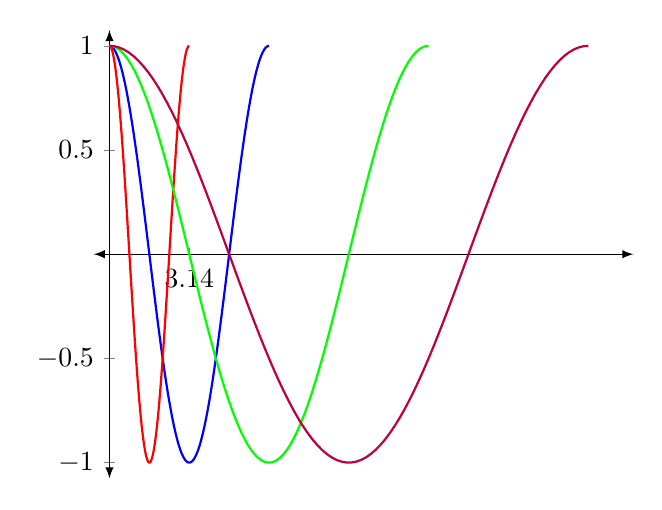
\begin{tikzpicture}
\begin{axis}[
    %axis equal image,
    axis lines=middle,
    xmin=0,xmax=20,
    ymin=-1,ymax=1,
    enlargelimits={abs=0.2cm},
    axis line style={latex-latex},
    ticklabel style={fill=white},
    ytick={-1,-0.5,0.5,1},
    xtick={-3.14, 3.14},
]
	% Draw the two parts separately with individual domains:
	\addplot[samples=100,domain=0:6.28, thick, color=blue] {cos(180/3.14*x)};
	\addplot[samples=100,domain=0:3.14, thick, color=red] {cos(2*180/3.14*x)};
	\addplot[samples=100,domain=0:12.56, thick, color=green] {cos(0.5*180/3.14*x)};
	\addplot[samples=100,domain=0:18.85, thick, color=purple] {cos(180/(3*3.14)*x)};
\end{axis}
\end{tikzpicture}
\end{marginfigure}

\subsection{Shifted Sine and Cosine Curves}
The sin/cos curves 
\begin{align*}
y = a\sin\bigg( k(x-b) \bigg) \qquad y = a\cos\bigg( k(x-b) \bigg) \qquad (k > 0)
\end{align*}
have \textbf{amplitude} $\abs{a}$, \textbf{period} $2\pi/k$, and \textbf{phase shift} $b$.

\subsection{Examples}
\begin{enumerate}
\item $y = \sin\left( x + \frac{\pi}{6} \right)$ {\color{blue} left shift by $\pi/6$} \\[5px]
\begin{marginfigure}
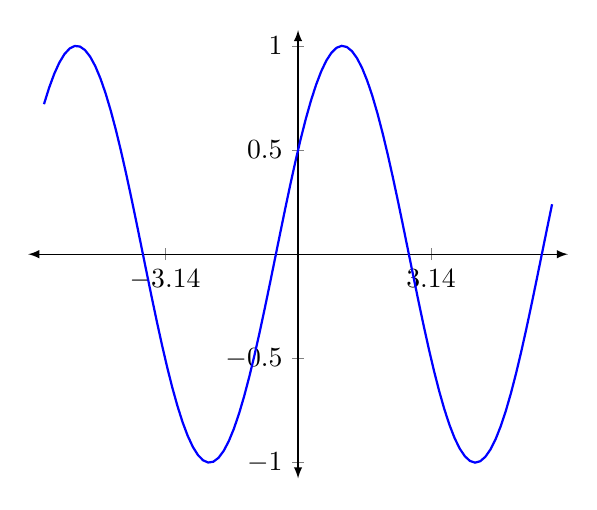
\begin{tikzpicture}
\begin{axis}[
    %axis equal image,
    axis lines=middle,
    xmin=-6,xmax=6,
    ymin=-1,ymax=1,
    enlargelimits={abs=0.2cm},
    axis line style={latex-latex},
    ticklabel style={fill=white},
    ytick={-1,-0.5,0.5,1},
    xtick={-3.14, 3.14},
]
	% Draw the two parts separately with individual domains:
	\addplot[samples=100,domain=-6:6, thick, color=blue] {sin(180/3.14*(x + 3.14/6))};
\end{axis}
\end{tikzpicture}
\end{marginfigure}

\item $y = 3\sin\left( 2\left( x - \frac{\pi}{4} \right) \right)$ {\color{blue} horizontal compression by 2, right shift by $\pi/4$, vertical stretch by 3} \\[5px]
\begin{marginfigure}
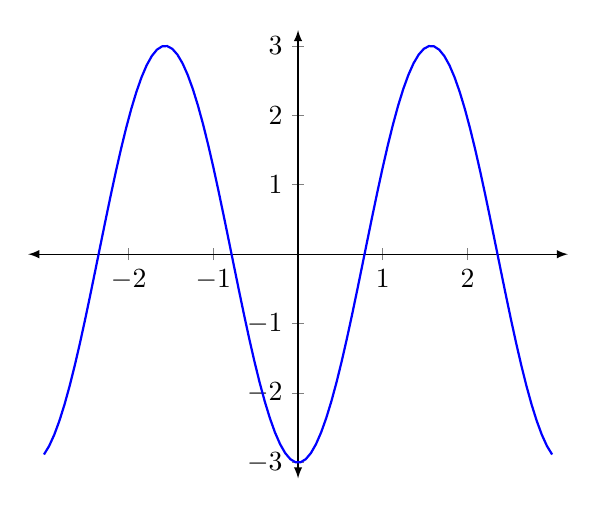
\begin{tikzpicture}
\begin{axis}[
    %axis equal image,
    axis lines=middle,
    xmin=-3,xmax=3,
    ymin=-3,ymax=3,
    enlargelimits={abs=0.2cm},
    axis line style={latex-latex},
    ticklabel style={fill=white},
    ytick={-3,-2,-1,1,2,3},
    xtick={-2,-1,1,2},
]
	% Draw the two parts separately with individual domains:
	\addplot[samples=100,domain=-3:3, thick, color=blue] {3*sin(2*180/3.14*(x - 3.14/4))};
\end{axis}
\end{tikzpicture}

\end{marginfigure}

\end{enumerate}

\section{Average value for sine and cosine}

On average what is the value for sine and cosine?  We could do integrals to figure it out but we don't know calculus here so we can guess.  Answer is zero.  So if you have a shift then the average is the shift.  Phase shift, period and amplitude don't affect it.

However, what if you compute the arc for sine and cosine?  Example: $\sin(2x)+3$ for $[0,\pi]$ and $[\frac{-\pi}{4},\frac{\pi}{4}]$

\subsection{Application problem}
\begin{enumerate}
\item The rate of intake during a respiratory cycle (liters/sec) for a person at rest is proportional to a sine wave with period six seconds. Suppose the rate is 0.85 liters/sec when t = 1.5 seconds. Write the sine equation that describes the rate of intake as a function of time

\item The following functions describes the air temperature in Fairbanks, Alaska as a function of time.

\begin{gather}
T(t) = 37 \sin(\frac{2\pi}{365}t - 1.7386) + 25
\end{gather}

\end{enumerate}


%%%%%%%%%%%%%%%%%%%%%%%%%%%%%%%%%%%%%%%%%%%%%%%%%%%%%%%%%%%%%%%%%%%%%%%%%%
%% -------------------------- SECTION 2 ----------------------------------
%%%%%%%%%%%%%%%%%%%%%%%%%%%%%%%%%%%%%%%%%%%%%%%%%%%%%%%%%%%%%%%%%%%%%%%%%%
\section{Section 5.4: More Trigonometric Graphs}

\subsection{Graphs of Tangent, Cotangent, Secant, and Cosecant}

\subsection{Periodic Properties}
\begin{enumerate}
\item tan and cot are $2\pi$ periodic
\begin{align*}
\tan(x + \pi) = \tan(x), \qquad \cot(x + \pi) = \cot(x)
\end{align*}
\item sec and csc are $2\pi$ periodic
\begin{align*}
\csc(x + 2\pi) = \csc(x), \qquad \sec(x + 2\pi) = \sec(x)
\end{align*}
\end{enumerate}

\subsection{Tangent}
Just look at 1 period, $(-\pi/2, \pi/2)$.
\begin{enumerate}
\item $\tan(x) = \sin(x)/\cos(x)$, and $\cos(\pm\pi/2) = 0$ (vertical asymptotes)
\item Since both sin, cos are positive on the interval $(0, \pi/2)$, then as $x \to (\pi/2)^-$, $\tan(x) \to +\infty$
\item Since sin is negative but cos is positive on $(-\pi/2, 0)$, then as $x\to(-\pi/2)^+$, $\tan(x) \to -\infty$
\end{enumerate}
\begin{minipage}{0.4\textwidth}
\begin{tabular}{r|l}
$x$ & $\tan(x)$ \\ \hline
0 & 0 \\
$\pi/6$ & $\frac{1/2}{\sqrt{3}{2}} = \frac{\sqrt{3}}{3} \approx 0.58$ \\
$\pi/4$ & $\frac{\sqrt{2}/2}{\sqrt{2}/2} = 1$ \\
$\pi/3$ & $\frac{\sqrt{3}/2}{1/2} = \sqrt{3} \approx 1.73$
\end{tabular}
\end{minipage}
\begin{minipage}{0.5\textwidth}
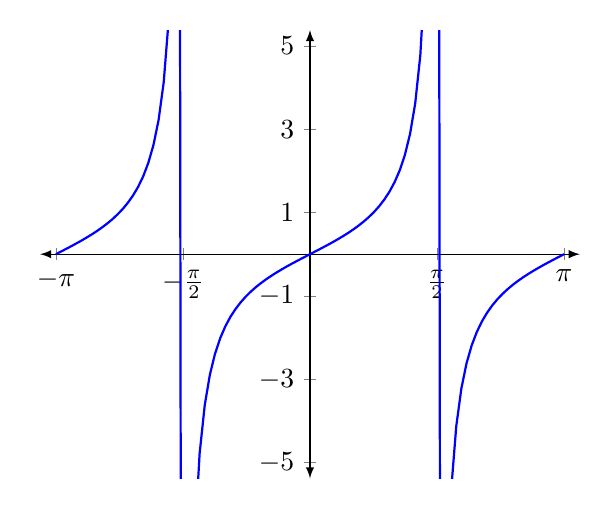
\begin{tikzpicture}
\begin{axis}[
    %axis equal image,
    axis lines=middle,
    xmin=-pi,xmax=pi,
    ymin=-5,ymax=5,
    enlargelimits={abs=0.2cm},
    axis line style={latex-latex},
    ticklabel style={fill=white},
    ytick={-5, -3, ..., 5},
    xtick={-3.14, -1.57, 1.57, 3.14},
    xticklabels={$-\pi$, $-\frac{\pi}{2}$, $\frac{\pi}{2}$, $\pi$},
]
	% Draw the two parts separately with individual domains:
	\addplot[samples=100,domain=-pi:pi, thick, color=blue] {tan(deg(x))};
\end{axis}
\end{tikzpicture}
\end{minipage}

\subsection{Cotangent}
Just look at 1 period, $(0, \pi)$.
\begin{enumerate}
\item $\cot(x) = \cos(x)/\sin(x)$, and $\sin(0) = \sin(\pi) = 0$ (vertical asymptotes)
\item Since both sin, cos are positive on the interval $(0, \pi/2)$, then as $x \to 0^+$, $\cot(x) \to +\infty$
\item Since sin is negative but cos is positive on $(\pi/2, \pi)$, then as $x\to \pi^-$, $\cot(x) \to -\infty$
\end{enumerate}
\begin{minipage}{0.4\textwidth}
\begin{tabular}{r|l}
$x$ & $\cot(x)$ \\ \hline
$\pi/6$ & $\frac{\sqrt{3}/2}{1/2} = \sqrt{3} \approx 1.73$ \\
$\pi/4$ & $\frac{\sqrt{2}/2}{\sqrt{2}/2} = 1$ \\
$\pi/3$ & $\frac{1/2}{\sqrt{3}{2}} = \frac{\sqrt{3}}{3} \approx 0.58$ \\
$\pi/2$ & 0
\end{tabular}
\end{minipage}
\begin{minipage}{0.5\textwidth}
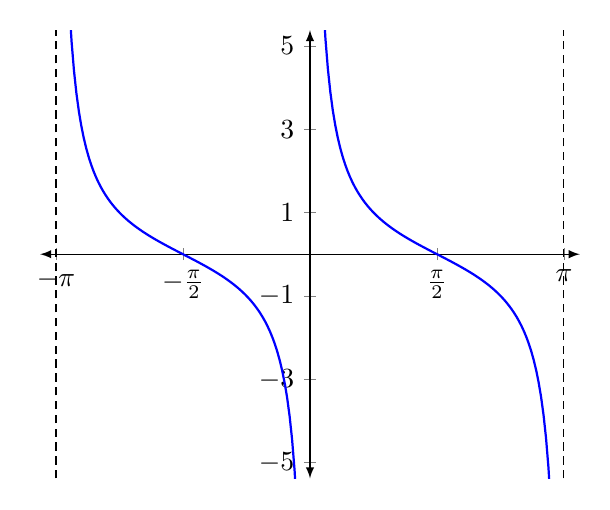
\begin{tikzpicture}
\begin{axis}[
    %axis equal image,
    axis lines=middle,
    xmin=-pi,xmax=pi,
    ymin=-5,ymax=5,
    enlargelimits={abs=0.2cm},
    axis line style={latex-latex},
    ticklabel style={fill=white},
    ytick={-5, -3, ..., 5},
    xtick={-3.14, -1.57, 1.57, 3.14},
    xticklabels={$-\pi$, $-\frac{\pi}{2}$, $\frac{\pi}{2}$, $\pi$},
    vasymptote=-3.14, 
    vasymptote=3.14
]
	% Draw the two parts separately with individual domains:
	\addplot[samples=100,domain=-3.1:-0.1, thick, color=blue] {cot(deg(x))};
	\addplot[samples=100,domain=0.1:3.1, thick, color=blue] {cot(deg(x))}; 
\end{axis}
\end{tikzpicture}
\end{minipage}

\begin{marginfigure}

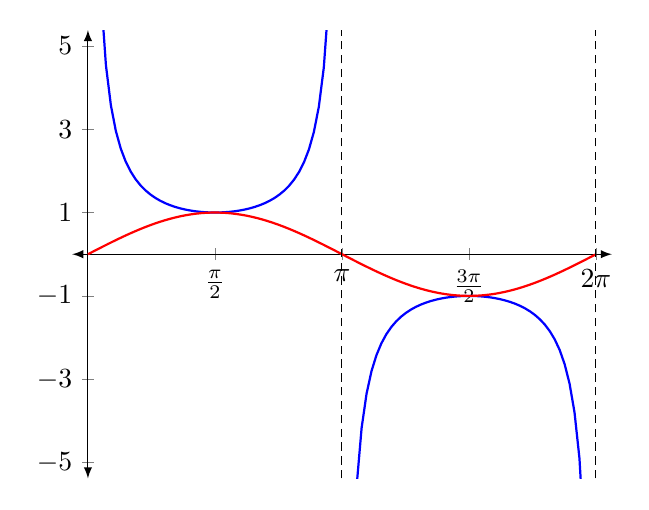
\begin{tikzpicture}
\begin{axis}[
    %axis equal image,
    axis lines=middle,
    xmin=0,xmax=2*pi,
    ymin=-5,ymax=5,
    enlargelimits={abs=0.2cm},
    axis line style={latex-latex},
    ticklabel style={fill=white},
    ytick={-5, -3, ..., 5},
    xtick={1.57, 3.14, 4.71, 6.28},
    xticklabels={$\frac{\pi}{2}$, $\pi$, $\frac{3\pi}{2}$, $2\pi$},
    vasymptote=3.14,
    vasymptote=6.28
]
	% Draw the two parts separately with individual domains:
	\addplot[samples=50,domain=0.1:3.1, thick, color=blue] {1/sin(deg(x))};
	\addplot[samples=50,domain=3.2:6.2, thick, color=blue] {1/sin(deg(x))};
	\addplot[samples=100,domain=0:2*pi, thick, color=red] {sin(deg(x))};
\end{axis}
\end{tikzpicture}

\end{marginfigure}

\subsection{Cosecant}
Just look at 1 period, $(0, 2\pi)$.
\begin{enumerate}
\item $\csc(x) = 1/\sin(x)$, and $\sin(n\pi) = 0$ (vertical asymptotes)
\end{enumerate}



\subsection{Secant}
Just look at 1 period, $(0, 2\pi)$.
\begin{enumerate}
\item $\sec(x) = 1/\cos(x)$, and $\cos(n\pi + \pi/2) = 0$ (vertical asymptotes)
\end{enumerate}
\begin{marginfigure}

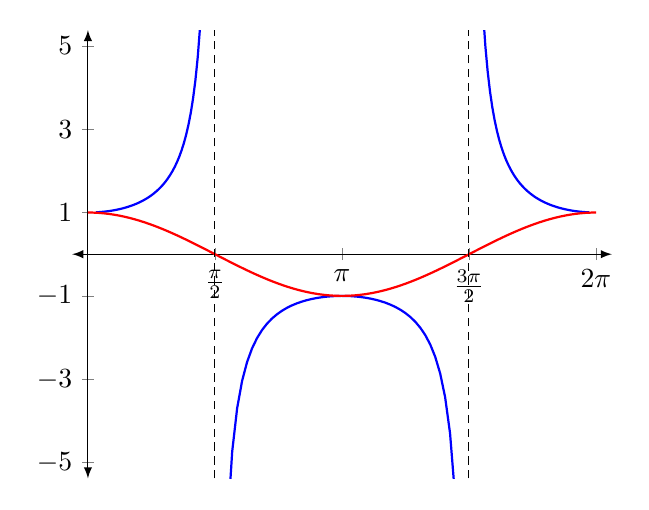
\begin{tikzpicture}
\begin{axis}[
    %axis equal image,
    axis lines=middle,
    xmin=0,xmax=2*pi,
    ymin=-5,ymax=5,
    enlargelimits={abs=0.2cm},
    axis line style={latex-latex},
    ticklabel style={fill=white},
    ytick={-5, -3, ..., 5},
    xtick={1.57, 3.14, 4.71, 6.28},
    xticklabels={$\frac{\pi}{2}$, $\pi$, $\frac{3\pi}{2}$, $2\pi$},
    vasymptote=1.57,
    vasymptote=4.71
]
	% Draw the two parts separately with individual domains:
	\addplot[samples=50,domain=0.1:1.5, thick, color=blue] {1/cos(deg(x))};
	\addplot[samples=50,domain=1.6:4.6, thick, color=blue] {1/cos(deg(x))};
	\addplot[samples=50,domain=4.8:6.2, thick, color=blue] {1/cos(deg(x))};
	\addplot[samples=100,domain=0:2*pi, thick, color=red] {cos(deg(x))};
\end{axis}
\end{tikzpicture}

\end{marginfigure}

\subsection{Graphs of Transformations of Tangent and Cotangent}

The functions 
\begin{align*}
y = a\tan(kx), \qquad y = a\cot(kx) \qquad (k > 0) 
\end{align*}
have period $\pi/k$. 
What about amplitude?
\begin{enumerate}
\item For tan, one period on $(-\pi/2k, \pi/2k)$
\item For cot, one period on $(0, \pi/k)$
\end{enumerate}

\subsection{Examples}
\begin{enumerate}
\item $y = \tan\left( 2 \left( x - \frac{\pi}{4} \right)\right)$ \\
\begin{minipage}{0.4\textwidth}
\begin{enumerate}
\item Horizontal compression by factor of 2, right shift by $\pi/4$
\item Start of period: 
\begin{align*}
2\left( x - \frac{\pi}{4} \right) = \frac{-\pi}{2} \Rightarrow
x - \frac{\pi}{4} = -\frac{\pi}{4} \Rightarrow
x = 0
\end{align*}
\item End of period: 
\begin{align*}
2\left( x - \frac{\pi}{4} \right) = \frac{\pi}{2} \Rightarrow
x - \frac{\pi}{4} = \frac{\pi}{4} \Rightarrow
x = \frac{\pi}{2}
\end{align*}
\end{enumerate}
\end{minipage}
\begin{minipage}{0.5\textwidth}
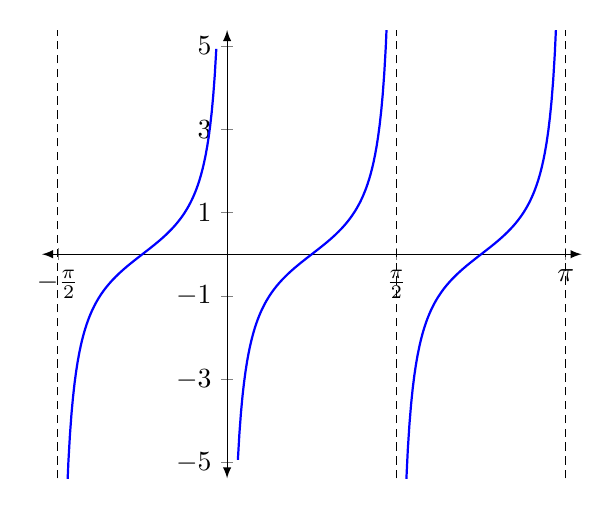
\begin{tikzpicture}
\begin{axis}[
    %axis equal image,
    axis lines=middle,
    xmin=-pi/2,xmax=pi,
    ymin=-5,ymax=5,
    enlargelimits={abs=0.2cm},
    axis line style={latex-latex},
    ticklabel style={fill=white},
    ytick={-5, -3, ..., 5},
    xtick={-1.57, 1.57, 3.14},
    xticklabels={$-\frac{\pi}{2}$, $\frac{\pi}{2}$, $\pi$},
    vasymptote=1.57,
    vasymptote=-1.57,
    vasymptote=3.14
]
	% Draw the two parts separately with individual domains:
	\addplot[samples=100,domain=-1.5:-0.1, thick, color=blue] {tan(deg(2*(x - pi/4)))};
	\addplot[samples=100,domain=0.1:1.5, thick, color=blue] {tan(deg(2*(x - pi/4)))};
	\addplot[samples=100,domain=1.6:3.1, thick, color=blue] {tan(deg(2*(x - pi/4)))};
\end{axis}
\end{tikzpicture}
\end{minipage}

\item $y = 2\cot\left( 3x - \frac{\pi}{2} \right) = 2\cot\left( 3\left( x - \frac{\pi}{6} \right) \right)$ \\
\begin{minipage}{0.4\textwidth}
\begin{enumerate}
\item Horizontal compression by factor 3, shift right $\pi/6$, vertical stretch by 2
\item Approximate period would be $(0/3, \pi/3)$ shift right $\left( 0 + \frac{\pi}{6}, \frac{\pi}{3} + \frac{\pi}{6} \right) = \left( \frac{\pi}{3}, \frac{\pi}{2} \right)$
\end{enumerate}
\end{minipage}
\begin{minipage}{0.5\textwidth}
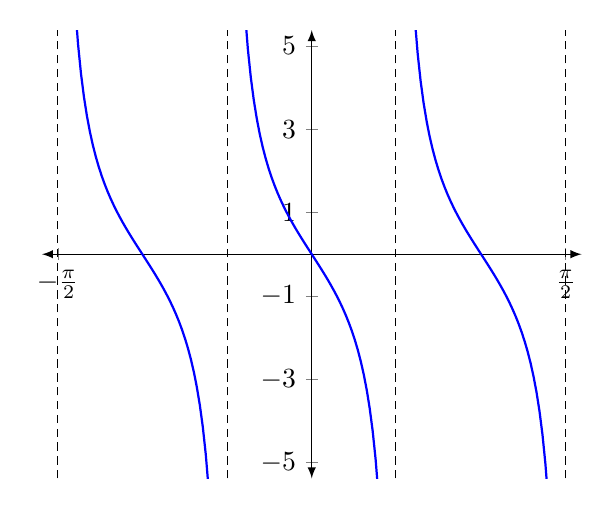
\begin{tikzpicture}
\begin{axis}[
    %axis equal image,
    axis lines=middle,
    xmin=-pi/2,xmax=pi/2,
    ymin=-5,ymax=5,
    enlargelimits={abs=0.2cm},
    axis line style={latex-latex},
    ticklabel style={fill=white},
    ytick={-5, -3, ..., 5},
    xtick={-1.57, 1.57, 3.14},
    xticklabels={$-\frac{\pi}{2}$, $\frac{\pi}{2}$, $\pi$},
    vasymptote=1.57,
    vasymptote=-1.57,
    vasymptote=0.52,
    vasymptote=-0.52
]
	% Draw the two parts separately with individual domains:
	\addplot[samples=50,domain=-1.5:-0.6, thick, color=blue] {2*cot(deg(3*(x - pi/6)))};
	\addplot[samples=50,domain=-0.45:0.45, thick, color=blue] {2*cot(deg(3*(x - pi/6)))};
	\addplot[samples=50,domain=0.6:1.5, thick, color=blue] {2*cot(deg(3*(x - pi/6)))};
\end{axis}
\end{tikzpicture}
\end{minipage}
\end{enumerate}

\subsection{Graphs of Transformations of Cosecant and Secant}
The functions
\begin{align*}
y = a\csc(kx), \qquad y = a\sec(kx) \qquad (k > 0)
\end{align*}
have period $2\pi/k$.
Appropriate interval for 1 complete period is $[0, 2\pi/k]$.

\subsection{Examples}

\begin{enumerate}
\item $y = \frac{1}{2} \csc\left( 2x + \frac{\pi}{2} \right) = \frac{1}{2} \csc\left( 2\left( x + \frac{\pi}{4} \right)\right)$ \\
\begin{minipage}{0.4\textwidth}
\begin{enumerate}
\item horizontal compression by 2, shift left by $\pi/4$, vertical compression by 2.
\item Start of period:
\begin{align*}
2x + \frac{\pi}{2} = 0 \Rightarrow 2x = -\frac{\pi}{2} \Rightarrow x= -\frac{\pi}{4}
\end{align*}
\item End of period:
\begin{align*}
2x + \frac{\pi}{2} = 2\pi \Rightarrow 2x = \frac{3\pi}{2} \Rightarrow x = \frac{3\pi}{4}
\end{align*}
\end{enumerate}
\end{minipage}
\begin{minipage}{0.5\textwidth}
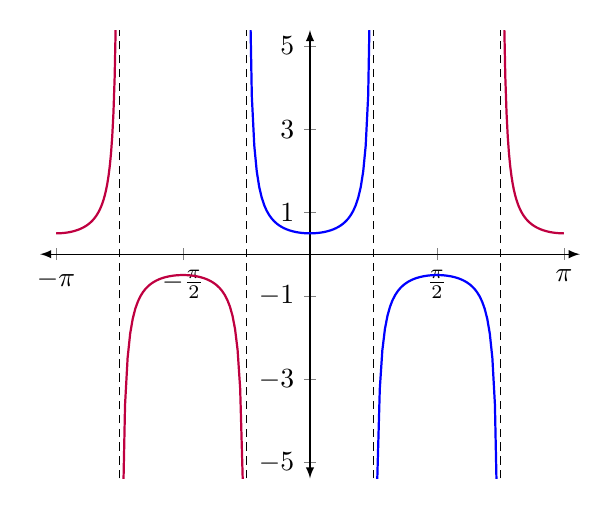
\begin{tikzpicture}
\begin{axis}[
    %axis equal image,
    axis lines=middle,
    xmin=-pi,xmax=pi,
    ymin=-5,ymax=5,
    enlargelimits={abs=0.2cm},
    axis line style={latex-latex},
    ticklabel style={fill=white},
    ytick={-5, -3, ..., 5},
    xtick={-3.14, -1.57, 1.57, 3.14},
    xticklabels={$-\pi$, $-\frac{\pi}{2}$, $\frac{\pi}{2}$, $\pi$},
    vasymptote=2.36,
    vasymptote=-2.36,
    vasymptote=0.78,
    vasymptote=-0.78
]
	% Draw the two parts separately with individual domains:
	\addplot[samples=50,domain=-0.75:0.75, thick, color=blue] {0.5/sin(deg(2*(x + pi/4)))};
	\addplot[samples=50,domain=0.8:2.35, thick, color=blue] {0.5/sin(deg(2*(x + pi/4)))};
	%\addplot[samples=50,domain=-1.57:-0.85, thick, color=blue] {0.5/sin(deg(2*(x + pi/4)))};
	
	\addplot[samples=50,domain=-2.35:-0.8, thick, color=purple] {0.5/sin(deg(2*(x + pi/4)))};
	%\addplot[samples=50,domain=1.57:2.3, thick, color=purple] {0.5/sin(deg(2*(x + pi/4)))};
	\addplot[samples=50,domain=-3.14:-2.4, thick, color=purple] {0.5/sin(deg(2*(x + pi/4)))};
	\addplot[samples=50,domain=2.4:3.14, thick, color=purple] {0.5/sin(deg(2*(x + pi/4)))};
	%\addplot[samples=50,domain=-0.45:0.45, thick, color=blue] {2*cot(deg(3*(x - pi/6)))};
	%\addplot[samples=50,domain=0.6:1.5, thick, color=blue] {2*cot(deg(3*(x - pi/6)))};
\end{axis}
\end{tikzpicture}
\end{minipage}

\item $y = 3 \sec\left( \frac{1}{2} x \right)$
\end{enumerate}

\end{document}